\documentclass{article}
\usepackage{graphicx} % Required for inserting images

\usepackage{tikz}
\usetikzlibrary{shapes.geometric, arrows}

% Presets, change here 
\tikzstyle{blue} = [rectangle, rounded corners, minimum width=3cm, minimum height=1cm,text centered, draw=black, fill=blue!30]
\tikzstyle{red} = [rectangle, rounded corners, minimum width=3cm, minimum height=1cm,text centered, draw=black, fill=red!30]
\tikzstyle{gold} = [rectangle, rounded corners, minimum width=3cm, minimum height=1cm,text centered, draw=black, fill=yellow!30]
\tikzstyle{goldenRod} = [rectangle, rounded corners, minimum width=3cm, minimum height=1cm,text centered, draw=black, fill=yellow!85]

\tikzstyle{arrow} = [thick,->,>=stealth]



\begin{document}
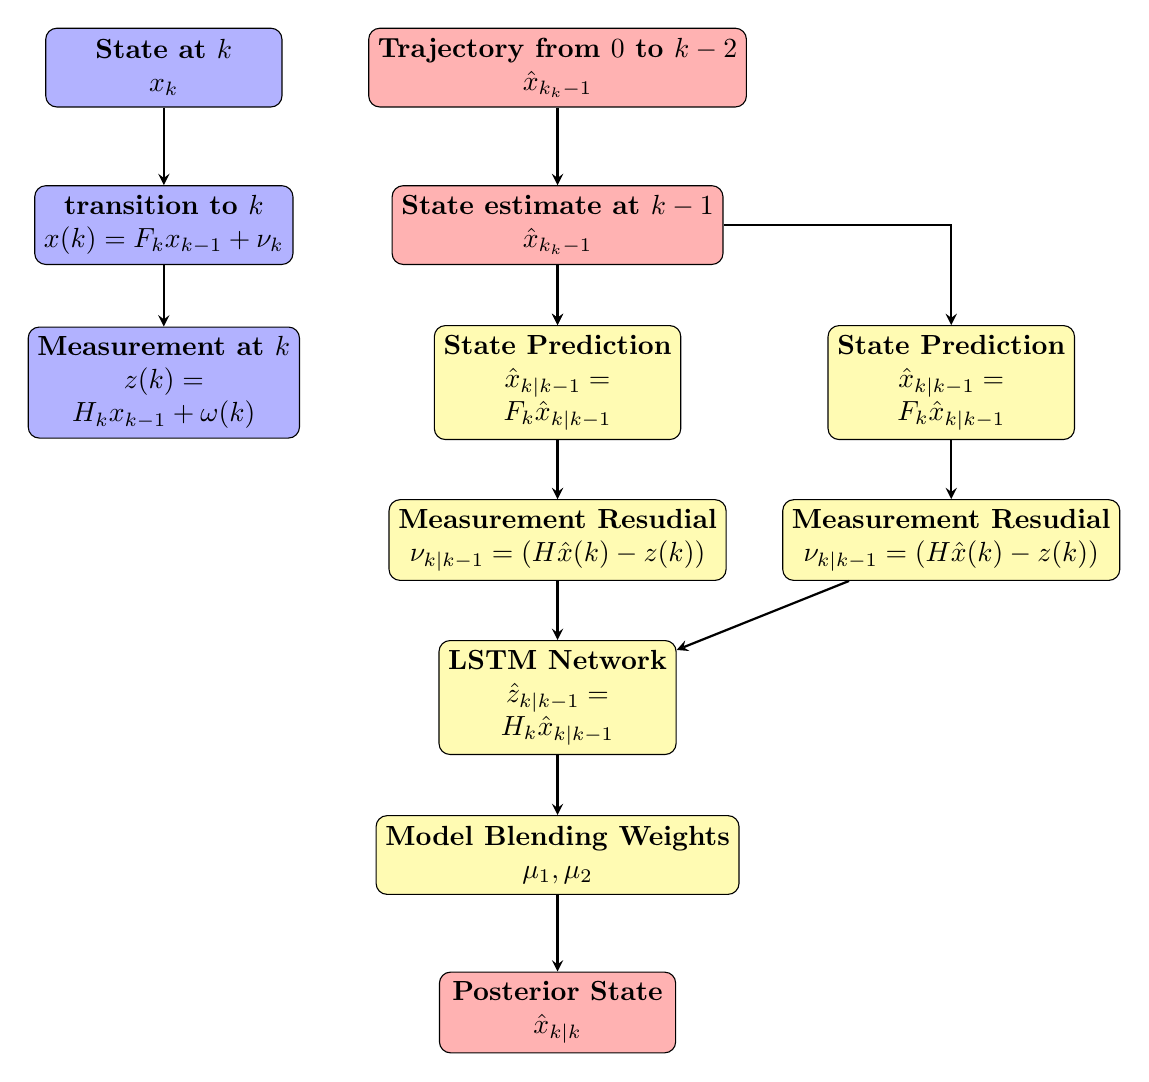
\begin{tikzpicture}[node distance=2cm]


%  Don't touch this          this is nickname     see presets above               The actual Text
% \node[draw, align=center]   (stateAT)          [blue]                      {\textbf{State at $t_k$} \\ $x(k)$};


% Column 1 - Evolution of the System (true state)
\node[draw, align=center] (stateAT) [blue] {\textbf{State at $k$} \\ $x_k$};
\node[draw, align=center] (transTO) [blue, below of=stateAT] {\textbf{transition to $k$} \\ $x(k) = F_k x_{k-1}+\nu_k$};
\node[draw, align=center] (measAT) [blue, below of=transTO] {\textbf{Measurement at $k$} \\ $z(k) = $\\$H_{k}x_{k-1} + \omega(k)$};

% Column 2 - Estimation of the State
\node[draw, align=center] (trajectoryEST) [red, right of=stateAT, xshift=3cm] {\textbf{Trajectory from $0$ to $k-2$} \\ $\hat{x}_{k_k-1}$};

\node[draw, align=center] (stateEST) [red, below of=trajectoryEST] {\textbf{State estimate at $k-1$} \\ $\hat{x}_{k_k-1}$};

\node[draw, align=center] (statePRED) [gold, below of=stateEST] {\textbf{State Prediction} \\ $\hat{x}_{k|k-1} =$ \\ $F_k\hat{x}_{k|k-1}$};

\node[draw, align=center] (MeasRed) [gold, below of=statePRED] {\textbf{Measurement Resudial} \\ $\nu_{k|k-1} = (H \hat{x}(k) - z(k))$};

\node[draw, align=center] (NeuralNetwork) [gold, below of=MeasRed] {\textbf{LSTM Network} \\ $\hat{z}_{k|k-1}=$ \\ $H_k\hat{x}_{k|k-1}$ };

\node[draw, align=center] (BlendWeights) [gold, below of=NeuralNetwork] {\textbf{Model Blending Weights} \\ $\mu_1, \mu_2$ };

\node[draw, align=center] (PosteriorState) [red, below of=BlendWeights] {\textbf{Posterior State} \\ $\hat{x}_{k|k}$ };


% Column 3 - Estimation of the State
\node[draw, align=center] (statePRED2) [gold, right of=statePRED, xshift=3cm] {\textbf{State Prediction} \\ $\hat{x}_{k|k-1} =$ \\ $F_k\hat{x}_{k|k-1}$};

\node[draw, align=center] (MeasRed2) [gold, below of=statePRED2] {\textbf{Measurement Resudial} \\ $\nu_{k|k-1} = (H \hat{x}(k) - z(k))$};


%  Don't touch this             From here        either --, |-, or -|                 to here
% \draw [arrow]             (stateAT)               --                               (transTO);

% Column 1 - Arrows
\draw [arrow] (stateAT) -- (transTO);
\draw [arrow] (transTO) -- (measAT);
%\draw [arrow] (measAT) |- (updateEST);

% Column 2 - Arrows
\draw [arrow] (stateEST) -- (statePRED);
\draw [arrow] (stateEST) -| (statePRED2);


\draw [arrow] (trajectoryEST) -- (stateEST);


\draw [arrow] (statePRED2) -- (MeasRed2);
\draw [arrow] (statePRED) -- (MeasRed);

\draw [arrow] (MeasRed) -- (NeuralNetwork);
\draw [arrow] (MeasRed2) -- (NeuralNetwork);


\draw [arrow] (NeuralNetwork) -- (BlendWeights);
%\draw [arrow] (statePRED) -- (measPRED);
%\draw [arrow] (measPRED) -- (updateEST);

\draw [arrow] (BlendWeights) -- (PosteriorState);

%Col 3 Arrows
\draw [arrow] (stateEST) -- (statePRED);

% Column 3 - Arrows
%\draw [arrow] (StateCov) -- (statePREDcov);
%\draw [arrow] (statePREDcov) -- (InnoCOV);
%\draw [arrow] (InnoCOV) -- (CrossCOV);
%\draw [arrow] (CrossCOV) -| (FilterG);
%\draw [arrow] (FilterG) -| (updateCOV);
%\draw [arrow] (FilterG) -| (updateEST);


\end{tikzpicture}




\end{document}